\documentclass{article}
\usepackage[utf8]{inputenc}
\usepackage[T1]{fontenc}
\usepackage{polski}
\usepackage{indentfirst}
\usepackage{lastpage}
\usepackage{fancyhdr}
\usepackage{graphicx}
\usepackage{listings}
\usepackage{caption}
\captionsetup[figure]{name={Rysunek}}

\pagestyle{fancy}
\fancyhf{}
\rhead{ Franciszek Wysocki, Bartosz Zdybel}
\rfoot{Strona \thepage \hspace{1pt} z \pageref{LastPage}}

\title{Specyfikacja Implementacyjna dla projektu pt. \\ ,,Gra w życie''}
\author{}
\date{}

\begin{document}
\maketitle

\begin{flushright}
\par ...
\vfill
\par
Wykonali: Franciszek Wysocki, Bartosz Zdybel

Sprawdzający: mgr inż. Paweł Zawadzki

Data: 08.03.2019
\end{flushright}

\thispagestyle{empty}
\newpage

% spis treści
\begin{frame}{}
    \tableofcontents
\end{frame}
\lhead{Spis treści}
\newpage

\section{Wstęp}
\lhead{Wstęp}

Dokument ten przedstawia szczegóły dotyczące implementacji projektu pt. ,,Gra w Życie'' oraz wytyczne dotyczące wersjonowania, środowiska, testów itd... (Więcej o działaniu opisane zostało w dokumencie ,,Specyfikacja funkcjonalna'').

\section{Informacje ogólne}
Program będzie zawierał interfejs tekstowy. Użytkownik nie będzie prowadził z nim dialogu, a wszystkie parametry będzie musiał podać przy uruchamianiu. Wymagane będzie podanie nazwy pliku wejściowego jako pierwszego argumentu wywołania z ewenetualnymi flagami. Program będzie domyślnie rysował pierwszą i ostatnią iterację (w przypadku braku podania ilości iteracji będzie wykonana tylko jedna).





\section{Środowisko deweloperskie}
Program będzie tworzony równolegle:
\begin{itemize}
\item na komputerze Dell Inspiron 5584 z procesorem Intel(R) Core(TM) i7-8565U CPU @ 1.80Ghz 1.99Ghz z zainstalowaną pamięcią RAM 16 GB działającym na systemie Windows 10 Home (Wersja 10.0.18362.657) z subsystemem (Windows subsystem for Linux) Ubuntu 18.04 LTS, (na którym będzie odbywać się kompilacja).
\item na komputerze Dell Vostro i7 z procesorem Intel(R) Core(TM) i7-8565U CPU @ 1.80Ghz 1.99Ghz z zainstalowaną pamięcia RAM 8 GB działającym na systemie Linux Ubuntu 18.04.
\end{itemize}

Kod będzie pisany w języku C (w standardzie ANSI).

\section{Zasady wersjonowania}

Wersjonowanie odbędzie się za pomocą gita (w formie dodanych tagów):

\begin{itemize}
\item
,,STABLE\_n'' - wersje stabilne, gdzie n = 1.0, 2.0, ...,
\item 
,,i'' - dla kolejnych wersji na głównej gałęzi i = n.1, n.2, ..., gdzie n to ostatnia wersja stabila (1, 2, ...) lub 0 jeżeli taka jeszcze nie istnieje,
\item
,,FINAL\_RELEASE'' - wesja finalna,
\end{itemize} 


Wiadomości z ,,commitów'' będą pisane w języku angielskim, a czasowniki będą występowały w formie gerund.

Np. Adding file operation (reading width, height, ...).

Praca na modułach będzie odbywać sie równolegle na gałęziach. Do scalania wykorzystywane będzie polecenie git merge.




\section{Moduły}

\subsection{Opis modułów}
W programie zostanie wyróżnionych 7 poniższych modułów:
\begin{itemize}
\item main - będzie odpowiadał za uruchomienie całej procedury (sterowanie)
\item control - będzie odpowiadał, za odczytanie flag i ich obsługę
\item input\_file - będzie odpowiadał za odczytanie danych z pliku wejściowego i sprawdzał jego poprawność
\item output\_file - będzie odpowiadał za zapisanie danych do pliku wyjściowego
\item board - będzie odpowiadał za utworzenie tablicy (siatki) na stercie i jej wypełnienie + będzie znajdować sie tam funkcja rysująca siatkę
\item png\_drawing - będzie odpowiadał za wygenerowanie obrazu o formacie png 
\item movement - moduł ten będzie podzielony na dwa mniejsze: moor i neumann, a dany z nich będzie uruchamiany w zależności od rodzaju sąsiedztwa, które użytkownik będzie chciał zastosować
\end{itemize}
\lhead{Moduły}
\subsection{Diagram modułów}
\begin{figure} [hbt!]
    \centering
    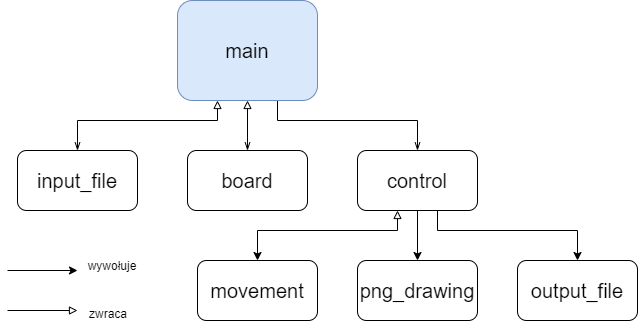
\includegraphics[width=12cm]{Untitled Diagram.png}
   \captionof{figure}{}
   % \captionof{}{caption 1}
\end{figure}


\newpage

\section{Argumenty wywołania}
\lhead{Argumenty wywołania}

Podczas uruchamiania będzie można korzystać tylko z poniższych flag w dowolnej kolejności:
\begin{itemize}
    \item \textbf{-SBS} 
    - Zostaną narysowane (na wyjściu standardowym) generacje w każdej iteracji,  
    \item \textbf{-N}
    - Zostanie wykonane n iteracji i wygenerowanie n +1 obrazów o formacie png (jeden z generacją inicjacyjną). Konieczny będzie kolejny argument (liczba n).
    \item \textbf{-S}
    - Zostanie nadpisany plik, do którego wpisany zostanie stan ostatniej generacji, tak aby plik ten mógł służyć jako plik wejściowy przy kolejnym uruchomieniu. Konieczny będzie kolejny argument (nazwa pliku).
\end{itemize}
Każdy inny argument (oprócz pierwszego, którym będzie nazwa pliku wejściowego) spowoduje zakończenie działania programu i wyświetlenie stosownego komunikatu.

\section{Testowanie}


Do każdego stworzonego modułu zostanie dodana 
jednostka testująca test\_nazwamodułu.c. 
Każdy z tych testów będzie miał możliwość kompilacji i uruchomienia bezpośrednio z programu make, wywołując ,,make test\_nazwamodułu.out". 
Testy będą niezależne od innych modułów.


\section{Struktury danych}
Wykorzystanie zostanie przede wszystkim tablica dwuwymiarowa na stercie, która będzie odwzorowaniem siatki ze stanem generacji.
%\newpage
\section{Algorytmy}
Wykorzystany zostanie wymyślony przez autorów algorytm stosowania sąsiedztwa na krawędziach i rogach. 
Istniejąca tablica ze sterty (Rysunek 2) będzie przepisywana do tymczasowej (tworzonej na nowo podczas każdej iteracji) tablicy poszerzonej o krawędź z każdej strony (Rysunek 3). 

\begin{figure} [hbt!]
    \centering
    
\includegraphics[width=3cm]{first.png}
    
    \captionof{figure}{}
\end{figure}

\begin{figure} [hbt!]
    \centering
    
\includegraphics[width=5.5cm]{second.png}
    
    \captionof{figure}{}
\end{figure}


\begin{figure} [hbt!]
    \centering
    
\includegraphics[width=5.5cm]{third.png}
    
    \captionof{figure}{}
\end{figure}

Każdy róg nowej siatki będzie odpowiadał naprzeciwległemu rogowi z istniejącej tablicy (Rysunek 4).
\newpage
Każda krawędź nowej siatki zostanie przepisana z naprzeciwległej krawędzi z istniejącej tablicy (Rysunek 5).
\begin{figure} [hbt!]
    \centering
    
\includegraphics[width=5.5cm]{fourth.png}
    \captionof{figure}{}
\end{figure}
\lhead{Algorytmy}
Funkcja odpowiadająca za ruch będzie zliczała ilość ,,żywych sąsiadów'' na tablicy tymczasowej (dla komórek nieznajdujących się w rogach i na krawędziach) i odrazu będzie modyfikowała tablicę na stercie zgodnie z zasadami gry i przyjętym rodzajem sąsiedztwa. 


\end{document}
